\section{Network Results}
\subsection{L1 and L2 Metrics}
% BEGIN: degree distribution and power law

% END: degree distribution and power law

\subsection{Betweenness Centrality}
% BEGIN: betweenness centrality
The examination of betweenness centrality in our bipartite network, as depicted in Figure~\ref{fig:bet_all},
reveals a Power Law Distribution, indicative of a scale-free structure. This implies the presence of a few central
nodes that act as pivotal connectors, while the majority of nodes exhibit lower betweenness centrality.

\begin{figure}[H]
    \centering
    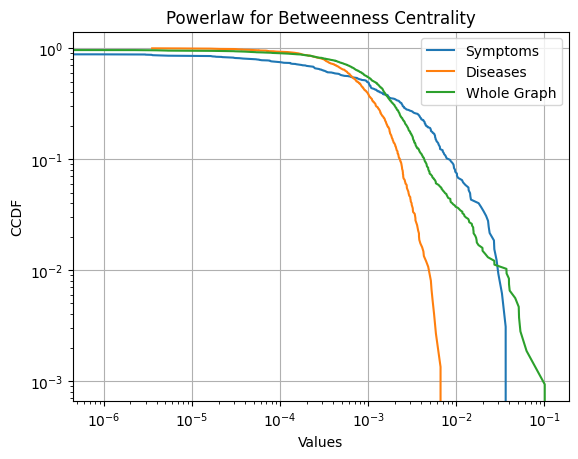
\includegraphics[width=\columnwidth]{bet_all.png}
    \caption{Betweenness Centrality CDFs}
    \label{fig:bet_all}
\end{figure}
\noindent
Upon dissecting the centrality values into symptoms and diseases (see Figures~\ref{fig:bet_diseases} and~\ref{fig:bet_symptoms}),
a notable observation emerges: symptoms tend to have higher betweenness centrality compared to diseases. To decipher the
significance of this result, it's essential to delve into the interpretation of betweenness centrality.

\begin{figure}[H]
    \centering
    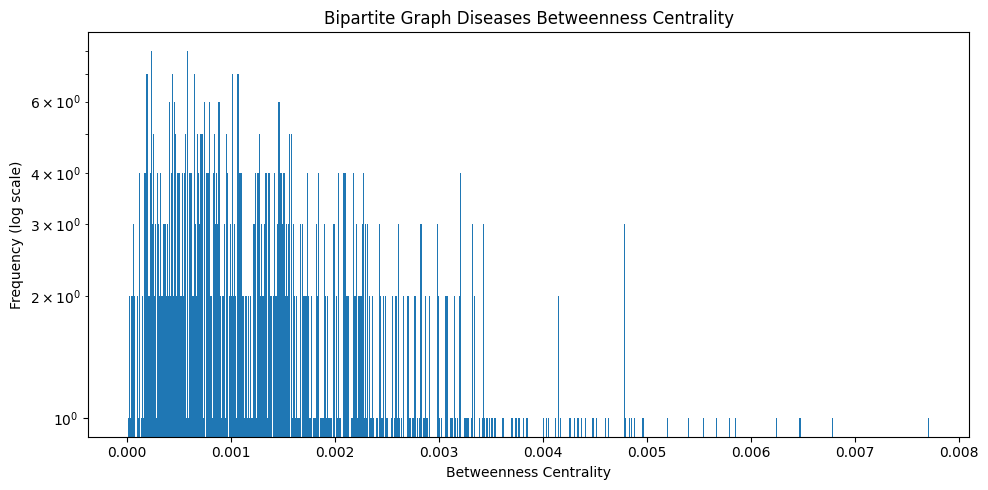
\includegraphics[width=\columnwidth]{bet_diseases.png}
    \caption{Betweenness Centrality of the diseases}
    \label{fig:bet_diseases}
\end{figure}
\noindent
\begin{figure}[H]
    \centering
    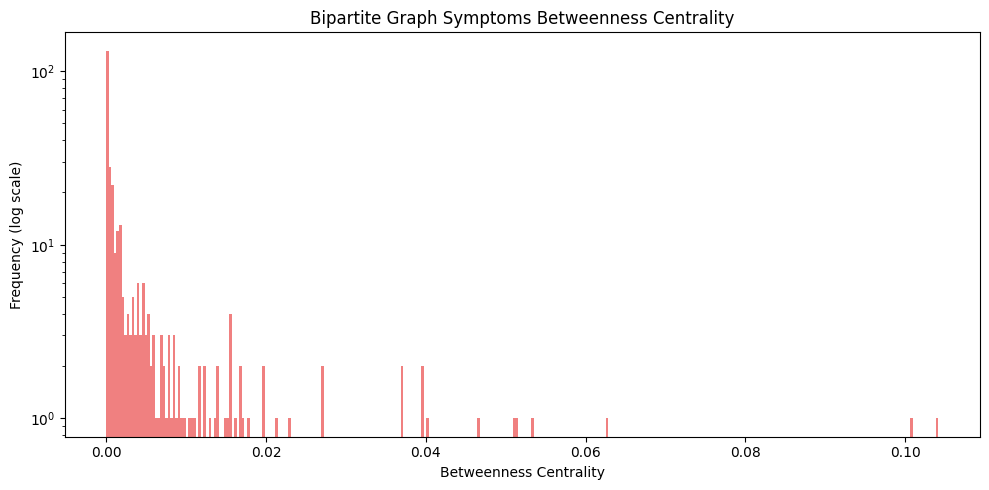
\includegraphics[width=\columnwidth]{bet_symptoms.png}
    \caption{Betweenness Centrality of the symptoms}
    \label{fig:bet_symptoms}
\end{figure}
\noindent
In general, a symptom exhibits high betweenness centrality when it is linked to numerous diseases, and these diseases,
in turn, are connected to a relatively limited set of symptoms. Conversely, a disease attains high betweenness centrality
when it connects to numerous symptoms, and these symptoms are associated with relatively few diseases.\\
Analyzing our results (L1 and L2), it becomes evident that the higher betweenness centrality of symptoms is attributed
to their connections with a multitude of diseases, while diseases, on the contrary, are linked to a relatively limited
number of symptoms. From a predictive standpoint, this outcome presents a challenge as each symptom is not sufficiently
specific, contributing to a broad array of disease classes.\\
Figure~\ref{fig:bet_top} highlights the top 10 nodes with the highest betweenness centrality, all of which are symptoms.
As anticipated, these symptoms are more generic in nature, aligning with their central role in connecting various diseases.

\begin{figure}[H]
    \centering
    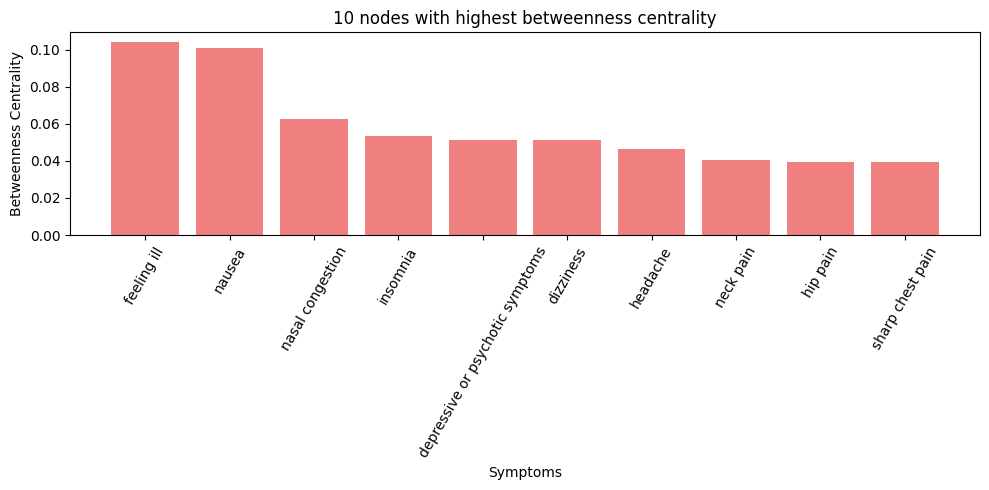
\includegraphics[width=\columnwidth]{bet_top.png}
    \caption{Top 10 nodes with the highest betweenness centrality}
    \label{fig:bet_top}
\end{figure}
\noindent
% END: betweenness centrality

\subsection{Communities}

% BEGIN: communities
The identification of communities within the network serves a dual purpose – facilitating network interpretation
and enhancing the capabilities of our ML prediction model.\\
From a network interpretation perspective, communities offer insights into disease-symptom relationships.
A community of symptoms signifies a set of symptoms that frequently co-occur within the same diseases, while a
community of diseases identifies a set of diseases often co-occurring within the same symptoms. The sizes of
different communities are illustrated in Figure~\ref{fig:com_sizes_all}.

\begin{figure}[H]
    \centering
    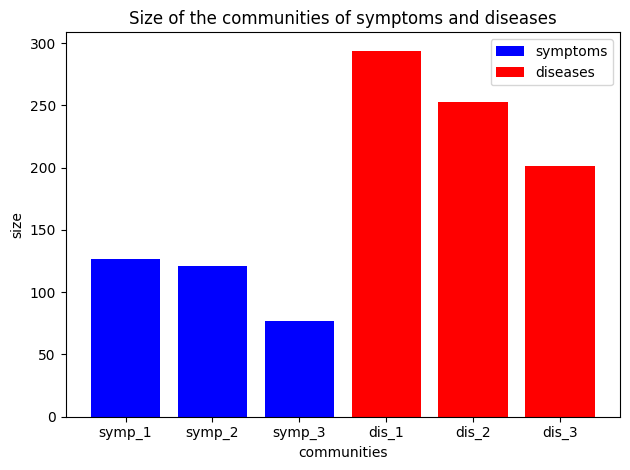
\includegraphics[width=\columnwidth]{com_sizes_all.png}
    \caption{Sizes of the communities of symptoms and diseases}
    \label{fig:com_sizes_all}
\end{figure}
\noindent
For clinical relevance, examining symptoms communities provides valuable information about diseases associated
with these symptoms. This is exemplified in Figures~\ref{fig:com1_symptoms}, \ref{fig:com2_symptoms},
and \ref{fig:com3_symptoms}. As an illustration, in the community 1 of symptoms (Figure~\ref{fig:com1_symptoms}),
'herniated disk' is the third most pointed disease by the symptoms of the community, with each symptom pointing,
on average, to three diseases.

\begin{figure}[H]
    \centering
    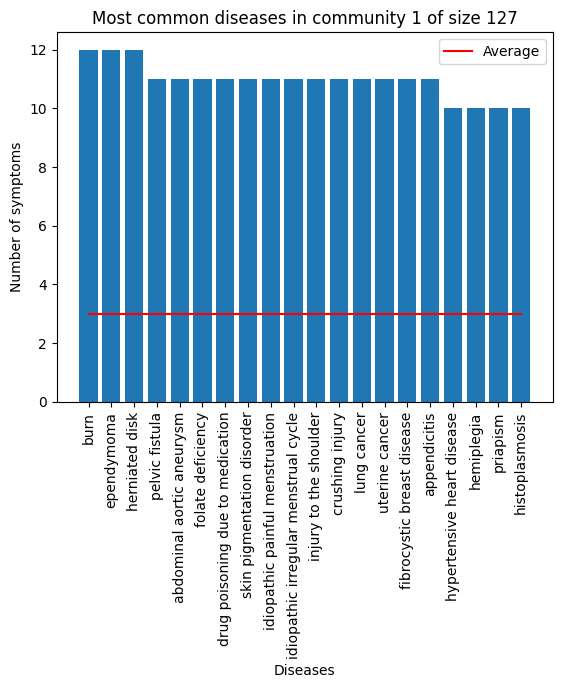
\includegraphics[width=\columnwidth]{com1_symptoms.png}
    \caption{Community 1 of symptoms}
    \label{fig:com1_symptoms}
\end{figure}
\noindent
A similar study can be conducted for communities of diseases, as depicted in Figures~\ref{fig:com1_diseases},
\ref{fig:com2_diseases}, and \ref{fig:com3_diseases}. This information aids in profiling diseases and understanding
the significance of each symptom. For instance, in community 1 of diseases (Figure~\ref{fig:com1_diseases}),
the symptom 'sharp abdominal pain' is present in almost half of the diseases in the community, indicating its
generic nature and limited discriminatory value.

\begin{figure}[H]
    \centering
    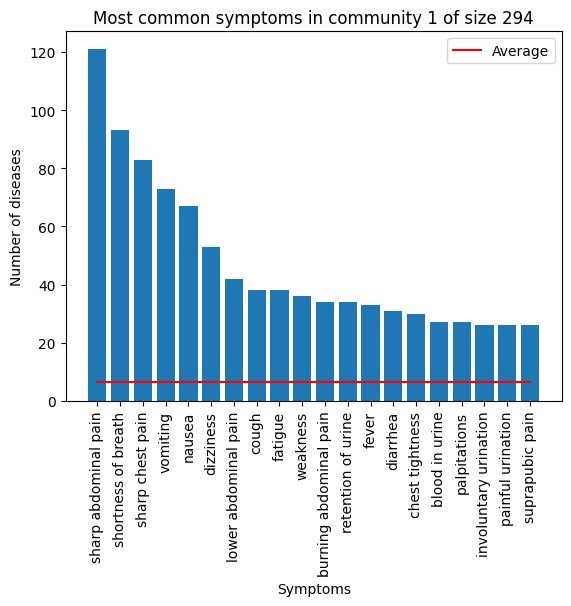
\includegraphics[width=\columnwidth]{com1_diseases.png}
    \caption{Community 1 of diseases}
    \label{fig:com1_diseases}
\end{figure}
\noindent
Transitioning to the creation of features for the ML model, two types of features were developed:\\

\begin{itemize}
    \setlength\itemsep{1em} % set space between items

    \item \textbf{Community Count:} This feature counts how many symptoms of the symptom vector belong to each community.
          Each symptom community is characterized by different pointed diseases. The model can learn to prioritize
          diseases associated with the community with the highest count.

    \item \textbf{Community Size:} This feature replaces each symptom in the symptom vector with the size of the
          community to which the symptom belongs. It enables the model to distinguish between symptoms belonging to small and
          large communities, injecting community information into the model beyond basic one-hot encoding of symptoms.
\end{itemize}
\noindent
\vspace{0.4cm}
It is noteworthy that communities can also contribute to improving the computational efficiency of the model.
For example, a symptom associated with many diseases may be less informative and could potentially be removed from the
symptom vector. However, we opted for a comprehensive approach using a combination of L1 and L2 measures to address this issue.

% END: communities

\subsection{Most Important Actors}
\label{subsec:most_important_actors}
% BEGIN: most important symptoms/diseases (4 classes)

As previously mentioned, our objective extends beyond feature extraction; we aim to leverage network information to
enhance the computational efficiency of the model. The strategy involves reducing the number of symptoms,
retaining only the most significant ones, to decrease training time while maintaining high accuracy.
Various approaches were tested, including L1, L2, betweenness centrality, and the degree of the unipartite projection
of symptoms. We performed a graphical analysis of their correlation (Figure \ref{fig:feat_corr}), favoring the
most uncorrelated features to provide the most complementary information.

\begin{figure*}[!t]
    \centering
    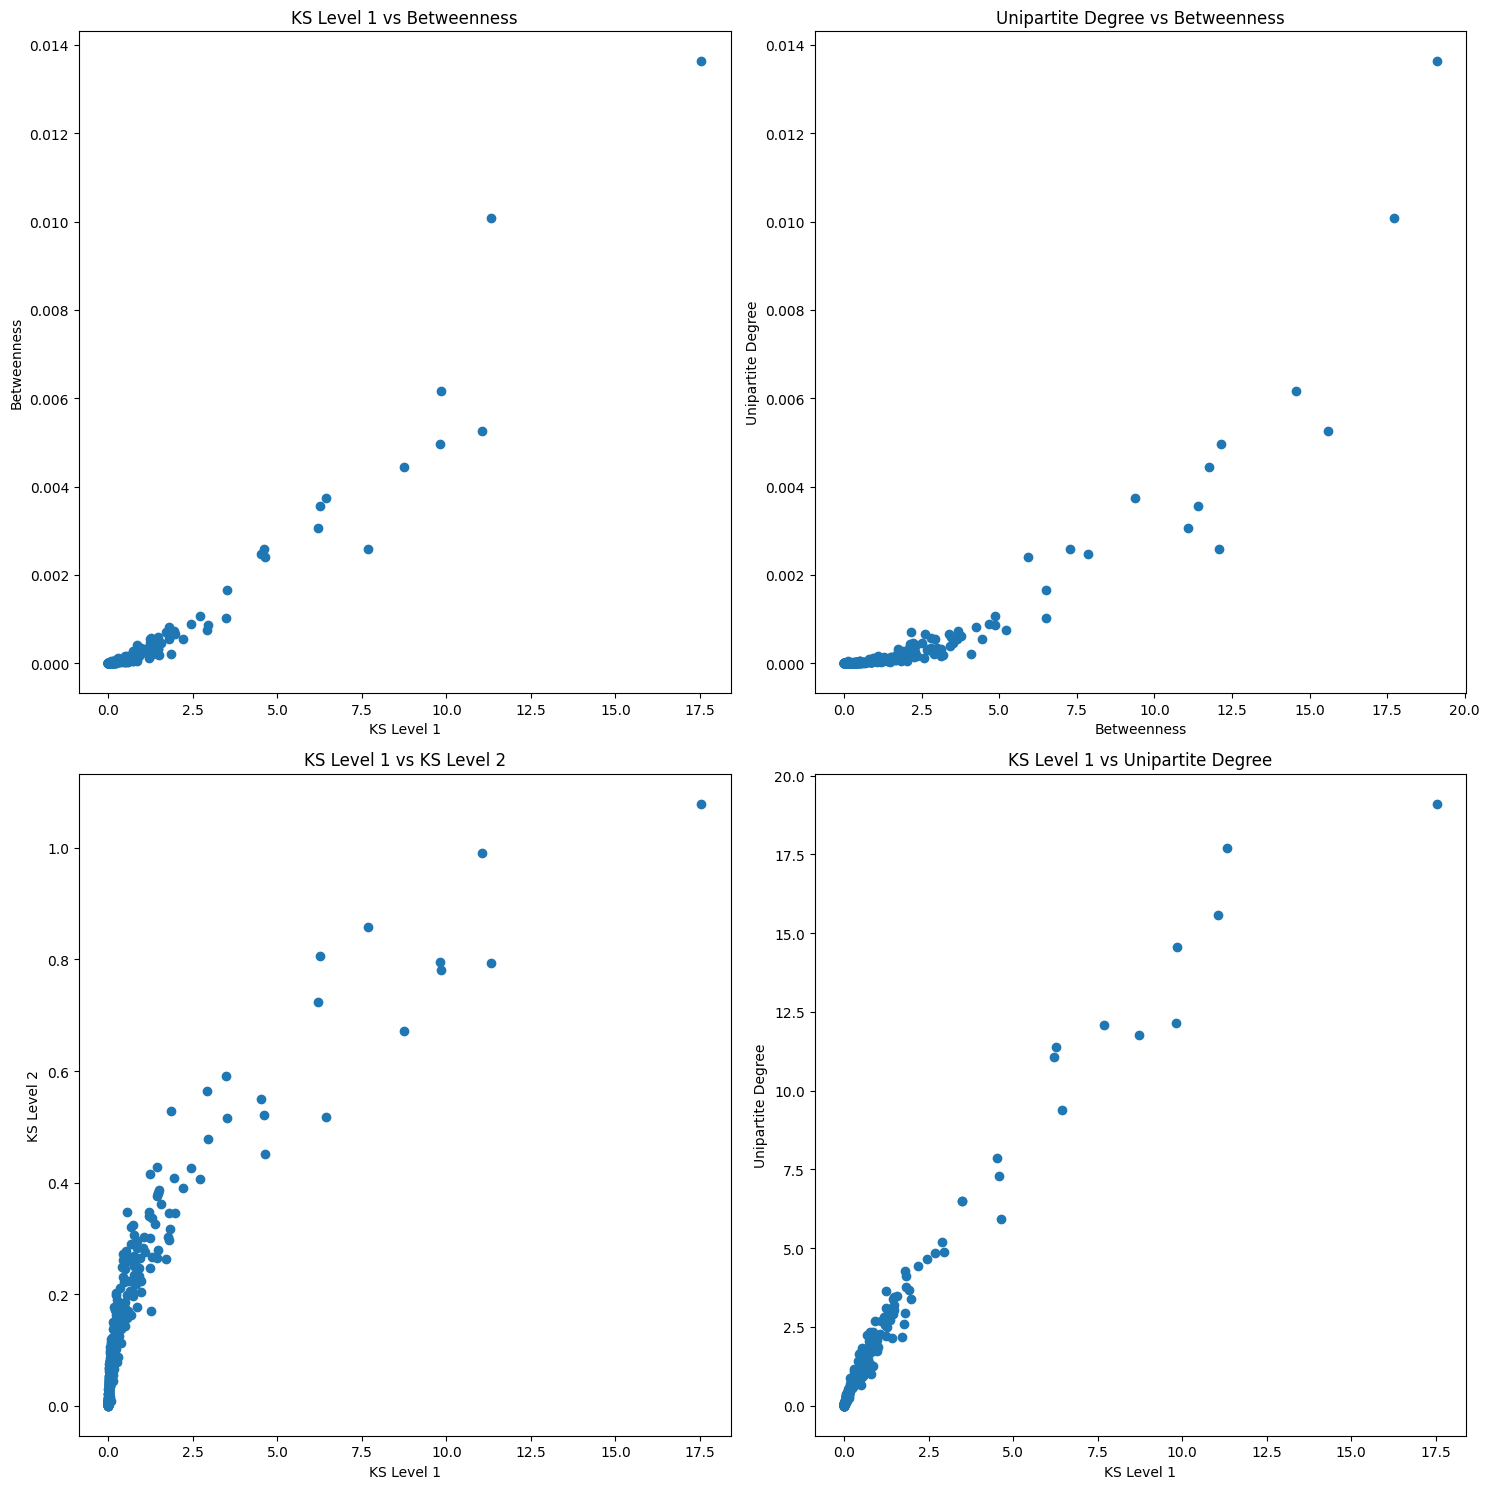
\includegraphics[width=\textwidth]{feat_corr.png}
    \caption{Correlation between features}
    \label{fig:feat_corr}
\end{figure*}

\noindent
Despite a non-negligible positive correlation in all cases, we opted for L1 and L2 due to their interpretability and
the less pronounced positive correlation at lower L1 values. This allows for a substantial division of symptoms for
the same value of L1 but different values of L2. Figure \ref{fig:l1_l2_division} illustrates the possibility of
placing a proper threshold on L1 and L2 to obtain four classes of symptoms, each with a non-null number of symptoms.

\begin{figure}[H]
    \centering
    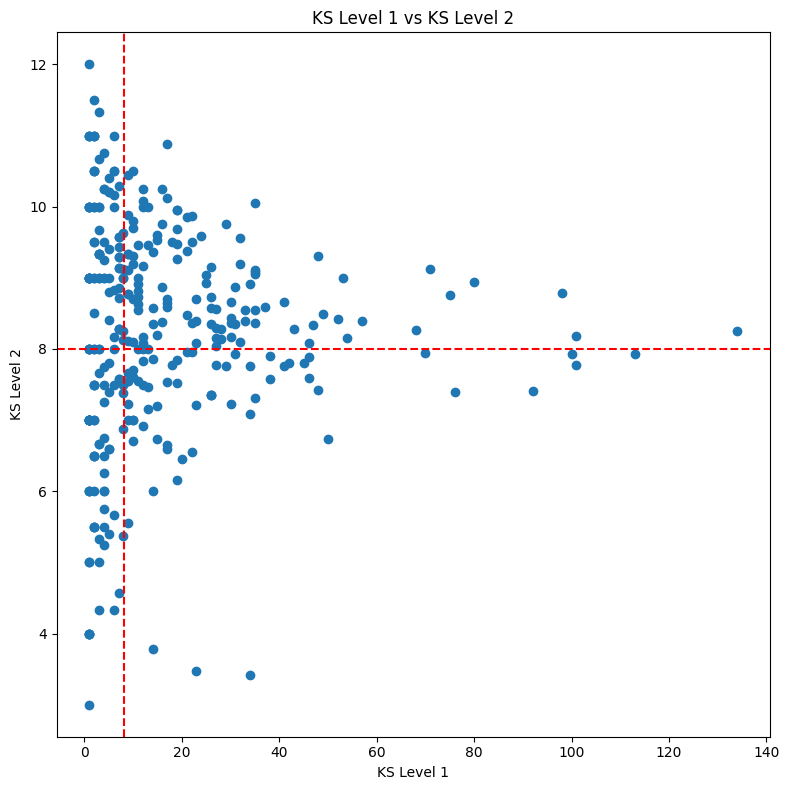
\includegraphics[width=\columnwidth]{l1_l2_division.png}
    \caption{Division based on L1 and L2 values}
    \label{fig:l1_l2_division}
\end{figure}
\noindent
To interpret these classes, we briefly recall the meanings of L1 and L2. The former represents the number of diseases
associated with a symptom, while the latter measures the number of symptoms associated with those diseases.
Consequently, we define the following classes:\\

\begin{itemize}
    \setlength\itemsep{1em}
    \item \textbf{High L1 - High L2}: Symptoms with high degree and high L2. These symptoms are less crucial for
          prediction as they contribute to many classes (diseases), which are also connected to many other symptoms.
    \item \textbf{High L1 - Low L2}: Symptoms with high degree and low L2. These symptoms should not be removed a
          priori since they can be useful. For instance, a symptom may be associated with many diseases, but those
          diseases may only be associated with that symptom. In this case, the symptom is very important for prediction.
    \item \textbf{Low L1 - High L2}: Symptoms with low degree and high L2. These symptoms may be important for
          prediction, as they contribute to few diseases.
    \item \textbf{Low L1 - Low L2}: Symptoms with low degree and low L2. These symptoms are the most important
          for prediction since they contribute to few classes (diseases), and those classes are also connected to
          few other symptoms.
\end{itemize}
\vspace{0.4cm}
\noindent
According to the above considerations, we can start from the last class and iteratively add symptoms from the
other classes, monitoring the impact on both accuracy and training time.
The results are analyzed in Section \ref{sec:results_ML}.\\
It is worth saying that all the other features (betweenness centrality, community count, and community size)
represent a valuable alternative to L1 and L2. Their use in computational time reduction is not explored in this work,
but it is a possible future development.

% END: most important symptoms/diseases (4 classes)



